\section{Testing / accuracy}
In order to see how the system performs in terms of accuracy, several tests have been conducted for the various implementations in the system. Since the system is dependent on good tuning and accurate sensor measurements to provide a good mapping of the maze, testing is very important. \\

I will test the range sensor, the edge detection algorithm and the mapping algorithm. When testing the edge detection and mapping, I will compare it to the work previously done in Bjørnsen 2016\cite{kris}. 

\subsection{Range sensor}
The range sensor measures the distance from the measuring device to a reflective object. The data collected from this sensor is used to determine the real life lengths of the walls in the maze.

\subsubsection{Setup}
The setup of the test is illustrated below. A measuring tape is placed along a surface, and the range sensor is placed at various distances along this measuring tape. At the end of the tape there is a straight wall that will reflect the sound waves.
\begin{figure}[H]
  \centering
  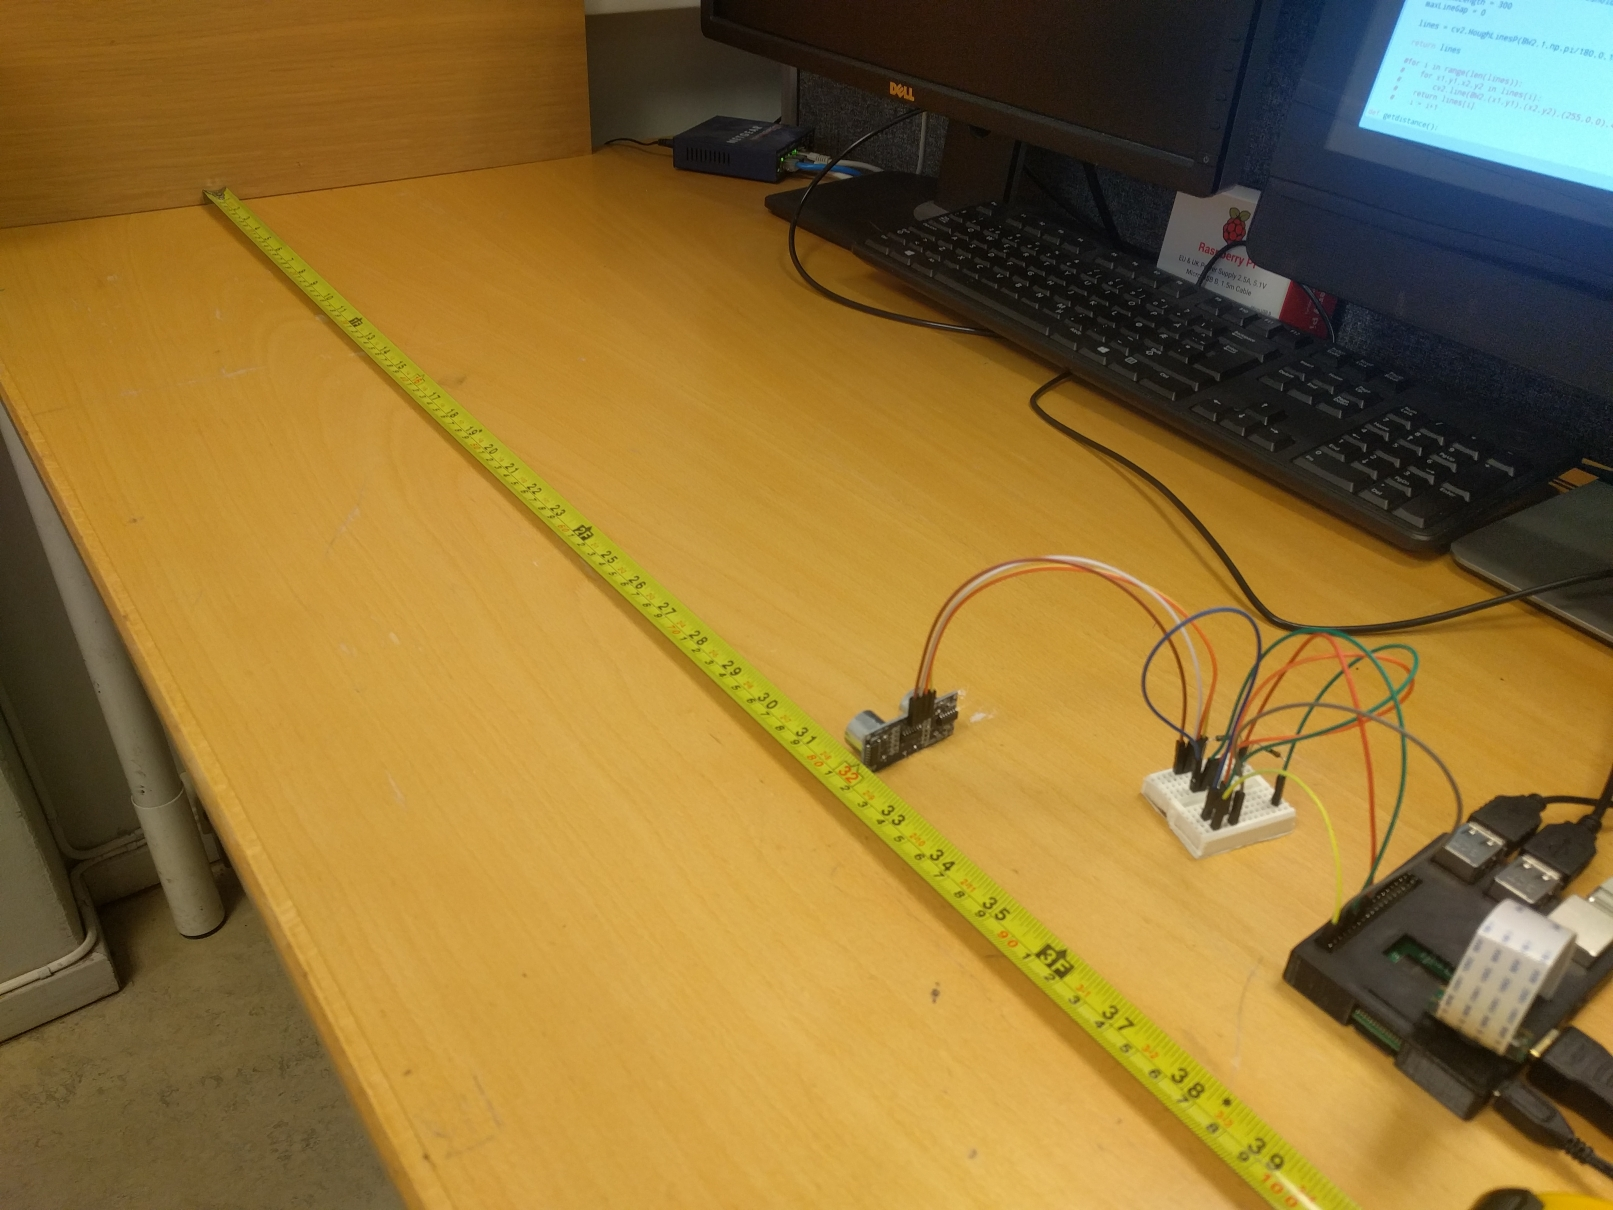
\includegraphics[width=0.7\textwidth]{fig/rangesetup}
  \caption{Range Sensor Setup}
  \label{fig:rsetup}
\end{figure}

\subsubsection{Measurements}
The following measurements were made for varying distances to the wall. The sensor was places such that the end of the two detectors were at the stated range. 


\begin{table}[H]
\centering
\begin{tabular}{|l|l|l|l|}
\hline
\textbf{Real Distance} & \textbf{Measured Distance} & \textbf{Diff} & \textbf{\% Diff} \\ \hline
40 cm                  & 39,12 cm                   & -0,88 cm       & 2,2           \\ \hline
50 cm                  & 48,96 cm                   & -1,04 cm       & 2,08           \\ \hline
60 cm                  & 59,12 cm                   & -0,88 cm       & 1,46           \\ \hline
70 cm                  & 69,03 cm                   & -0,97 cm       & 1,38           \\ \hline
80 cm                  & 78,8 cm                    & -1,2 cm        & 1,5            \\ \hline
90 cm                  & 88,46 cm                   & -1,54 cm       & 1,7           \\ \hline
100 cm                 & 98,53 cm                   & -1,47 cm       & 1,47          \\ \hline
110 cm                 & 108,9 cm                   & -1,1 cm        & 1           \\ \hline
120 cm                 & 118,63 cm                  & -1,37 cm       & 1,1          \\ \hline
\end{tabular}
\caption{Range sensor measurements}
\label{rangemeasurements}
\end{table}
The measurements range from 40 to 120 cm from the measured object. The difference in the measurements range from $0,88$ cm to $1,54$ cm. In terms of percentages in differences, the range was from $2,2\%$ to $1\%$. What is interesting, is that the actual difference seems to be about the same with varying distances. This means that there might be a "steady state" error which can be corrected for all distances by adding the mean of the differences to the measurement.

\begin{align*}
\textbf{Average Diff} = \frac{0,88+1,04+0,88+0,97+1,2+1,54+1,47+1,1+1,37}{9} = 1,1611\quad [cm]
\end{align*}

This value is added to the measurements to improve the average estimation of the distance from the system to the ground. One could argue that since the system is not intended to be used at heights lower than 50 cm, the mean could be calculated from a different range to get a better estimate.\\

The code for the Range sensor test is included in the Appendix.
\newpage


\subsection{Canny Edge detection}
An implementation of edge detection was developed in Bjørnsen 2016\cite{kris}, and to determine the feasibility of the newly implemented edge detection in Python it is beneficial to compare these two implementations with the same input. Since the implementations of the Canny edge algorithm is not entirely similar in OpenCV and in the Image Processing Toolbox in MATLAB, I have attempted to run them with the most similar thresholds and parameters as possible.

\subsubsection{Setup}
From Bjørnsen 2016\cite{kris}, we have the following test maze:
\begin{figure}[H]
\centering
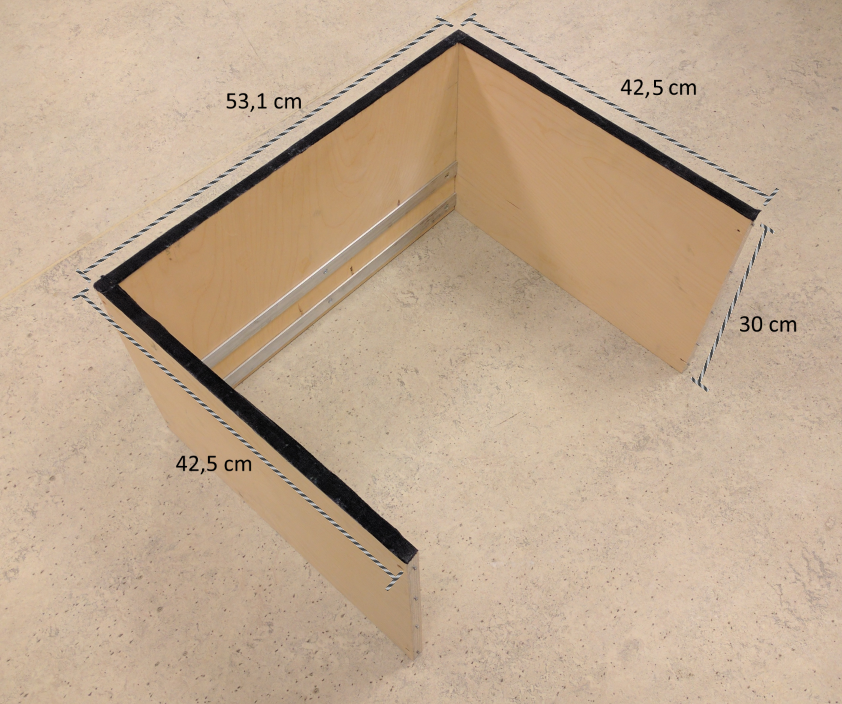
\includegraphics[width=0.9\textwidth]{fig/maze}
  \caption{Test maze}
  \label{fig:maze}
\end{figure}
Many images was taken of this maze using the Sony Exmor IMX377 in the project thesis, and since I am only testing for the edge detection aspect of the implementation; I can use the same images and compare both implementations. The image I am going to compare the edge detection implementations on is the following:

\begin{figure}[H]
\centering
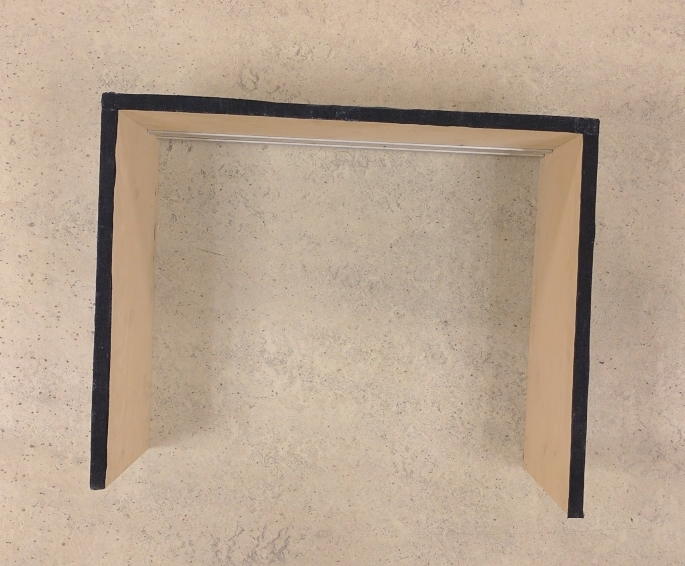
\includegraphics[width=0.7\textwidth]{fig/edgetest}
  \caption{Test Image}
  \label{fig:maze}
\end{figure}

The image was taken during the fall in Bjørnsen 2016\cite{kris}. The picture was taken on a tripod facing straight down as described in the project report.\\

What I am testing for here is a complete edge detection along all the walls of the test maze in the picture. There should be no other edges detected other than the top of the walls and it should be continuous with no holes along the edges.\\

The software that I used to test the edge detection is included in the appendix.

\subsubsection{Results}

\begin{figure}[H]
\centering
  \centering
  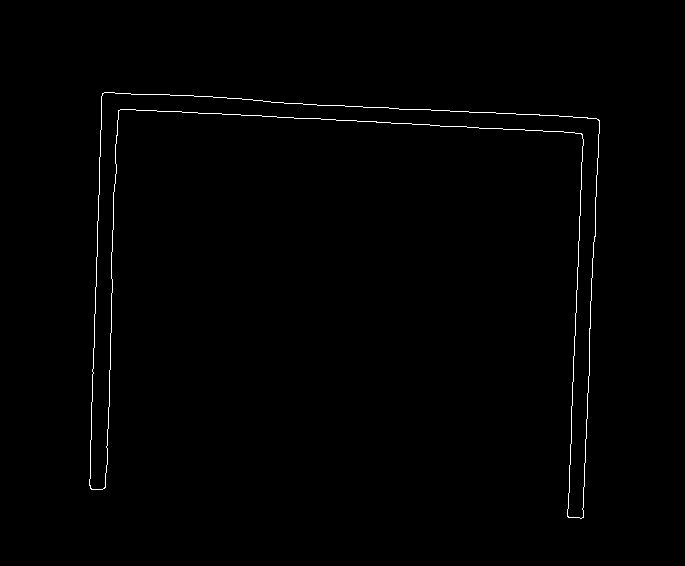
\includegraphics[width=0.7\textwidth]{fig/edge1}
  \caption{MATLAB Image Processing Toolbox Canny Implementation}
\end{figure}

\begin{figure}[H]
  \centering
  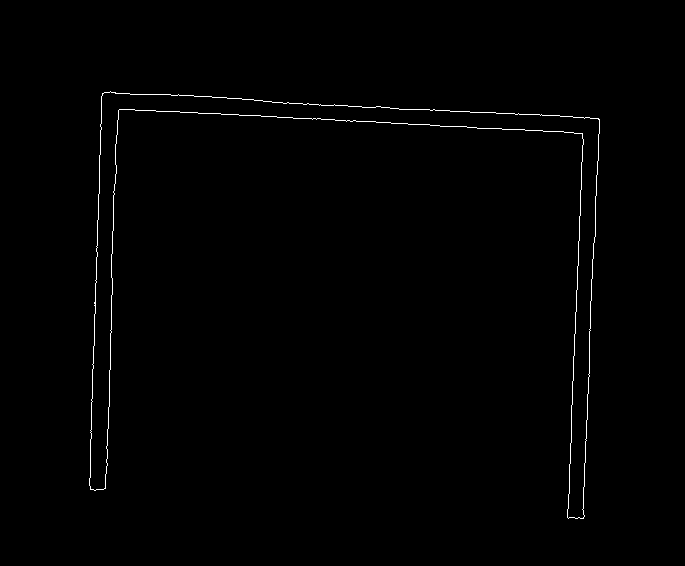
\includegraphics[width=0.7\textwidth]{fig/edge2}
  \caption{Python OpenCV Canny Implementation}
\end{figure}

The results show that with similar tuned threshold variables, the Python OpenCV implementation provides a complete edge detection, similar to that of the MATLAB implementation. 

\subsection{Mapping}
What I want my system to provide is the start- and end coordinates (x,y) of each wall segment detected with relation to where the system is positioned. Since I have not implemented any positioning, it is assumed that the system is in coordinates (0,0,90) where 90 is the theta angle, and all the walls are mapped relating to this position. This translates directly to the image center, since the image is captured normal to the ground plane.\\

There are a couple of factors I want to test with regards to the mapping implementation:
\begin{itemize}
\item Accuracy of mapping with accurate height measurement
\item Sensitivity to error in height measurements
\item Accuracy of mapping with varying heights
\end{itemize}

Some of these elements were tested for in Bjørnsen 2016\cite{kris}, and I intend to compare how this implementation behaves compared to that done previously. 

\subsubsection{Setup}
The setup in the different mapping test uses the test maze described previously, in addition to other elements. I have rigged the Raspberry Pi on a tripod facing normally to the ground plane. The power and ethernet cable is connected to the Raspberry Pi running up the tripod, and the Raspberry Pi is controlled remotely through the Remote Desktop Connection application in Windows as described earlier.\\

With this setup, many different tests can be conducted for testing the varying system pieces. The setup is built to replicate the state of which the system might find itself being mounted on a drone flying above a maze.

\begin{figure}[H]
\centering
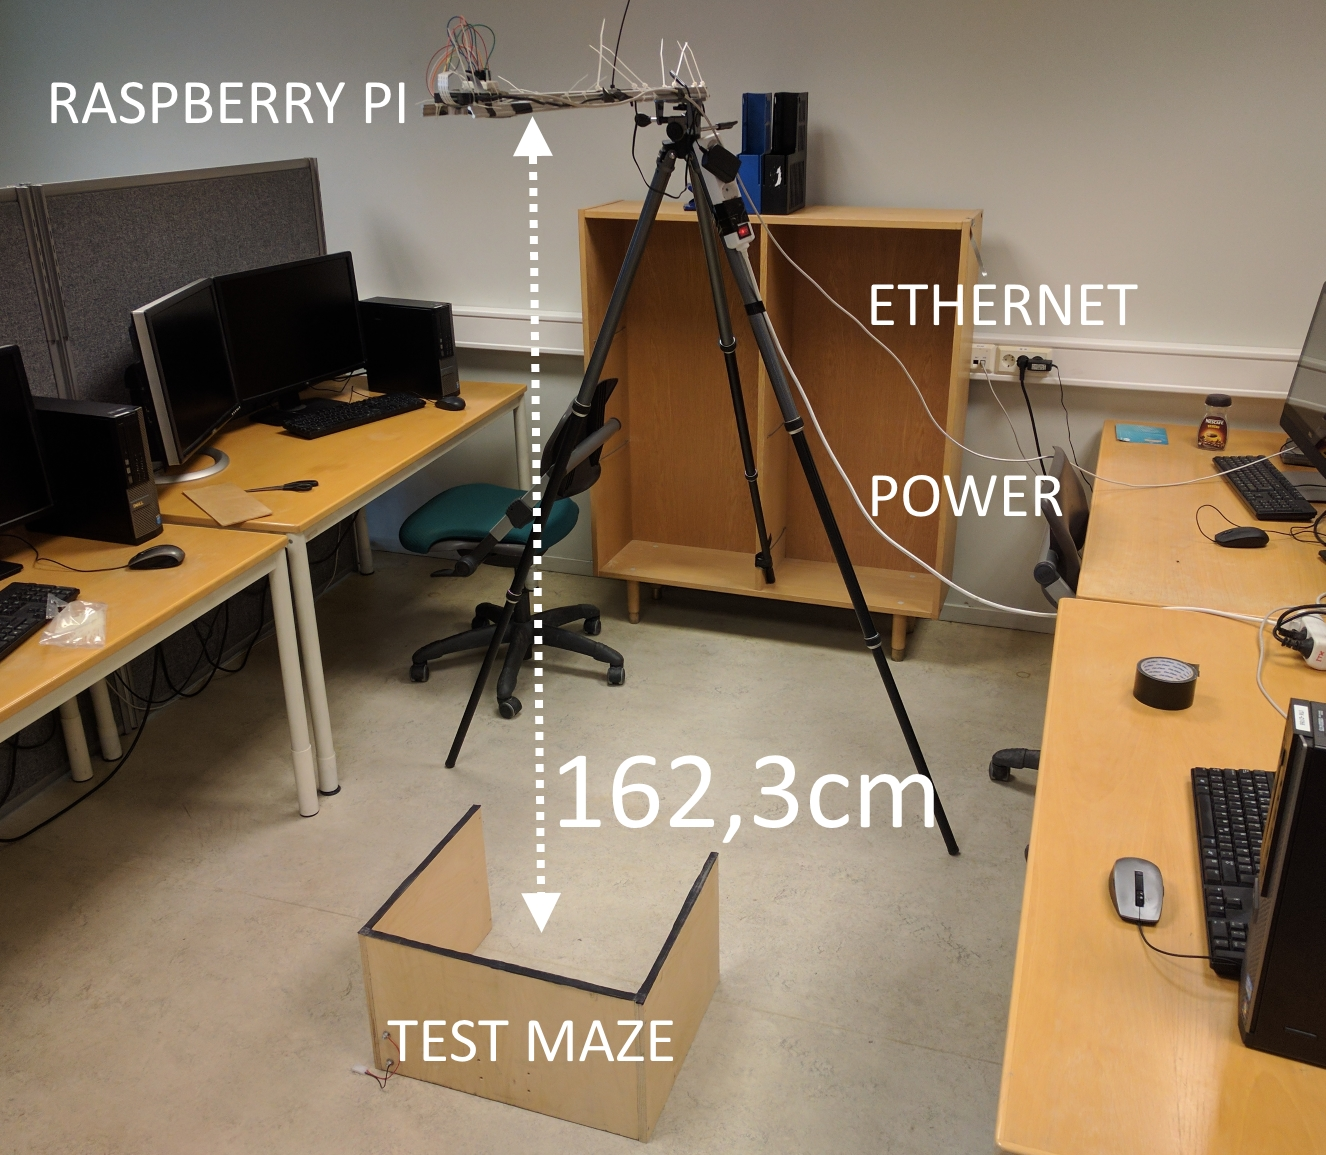
\includegraphics[width=0.8\textwidth]{fig/mapping_setup}
  \caption{Tripod setup used for testing}
  \label{fig:tripod}
\end{figure}
\begin{figure}[H]
\centering
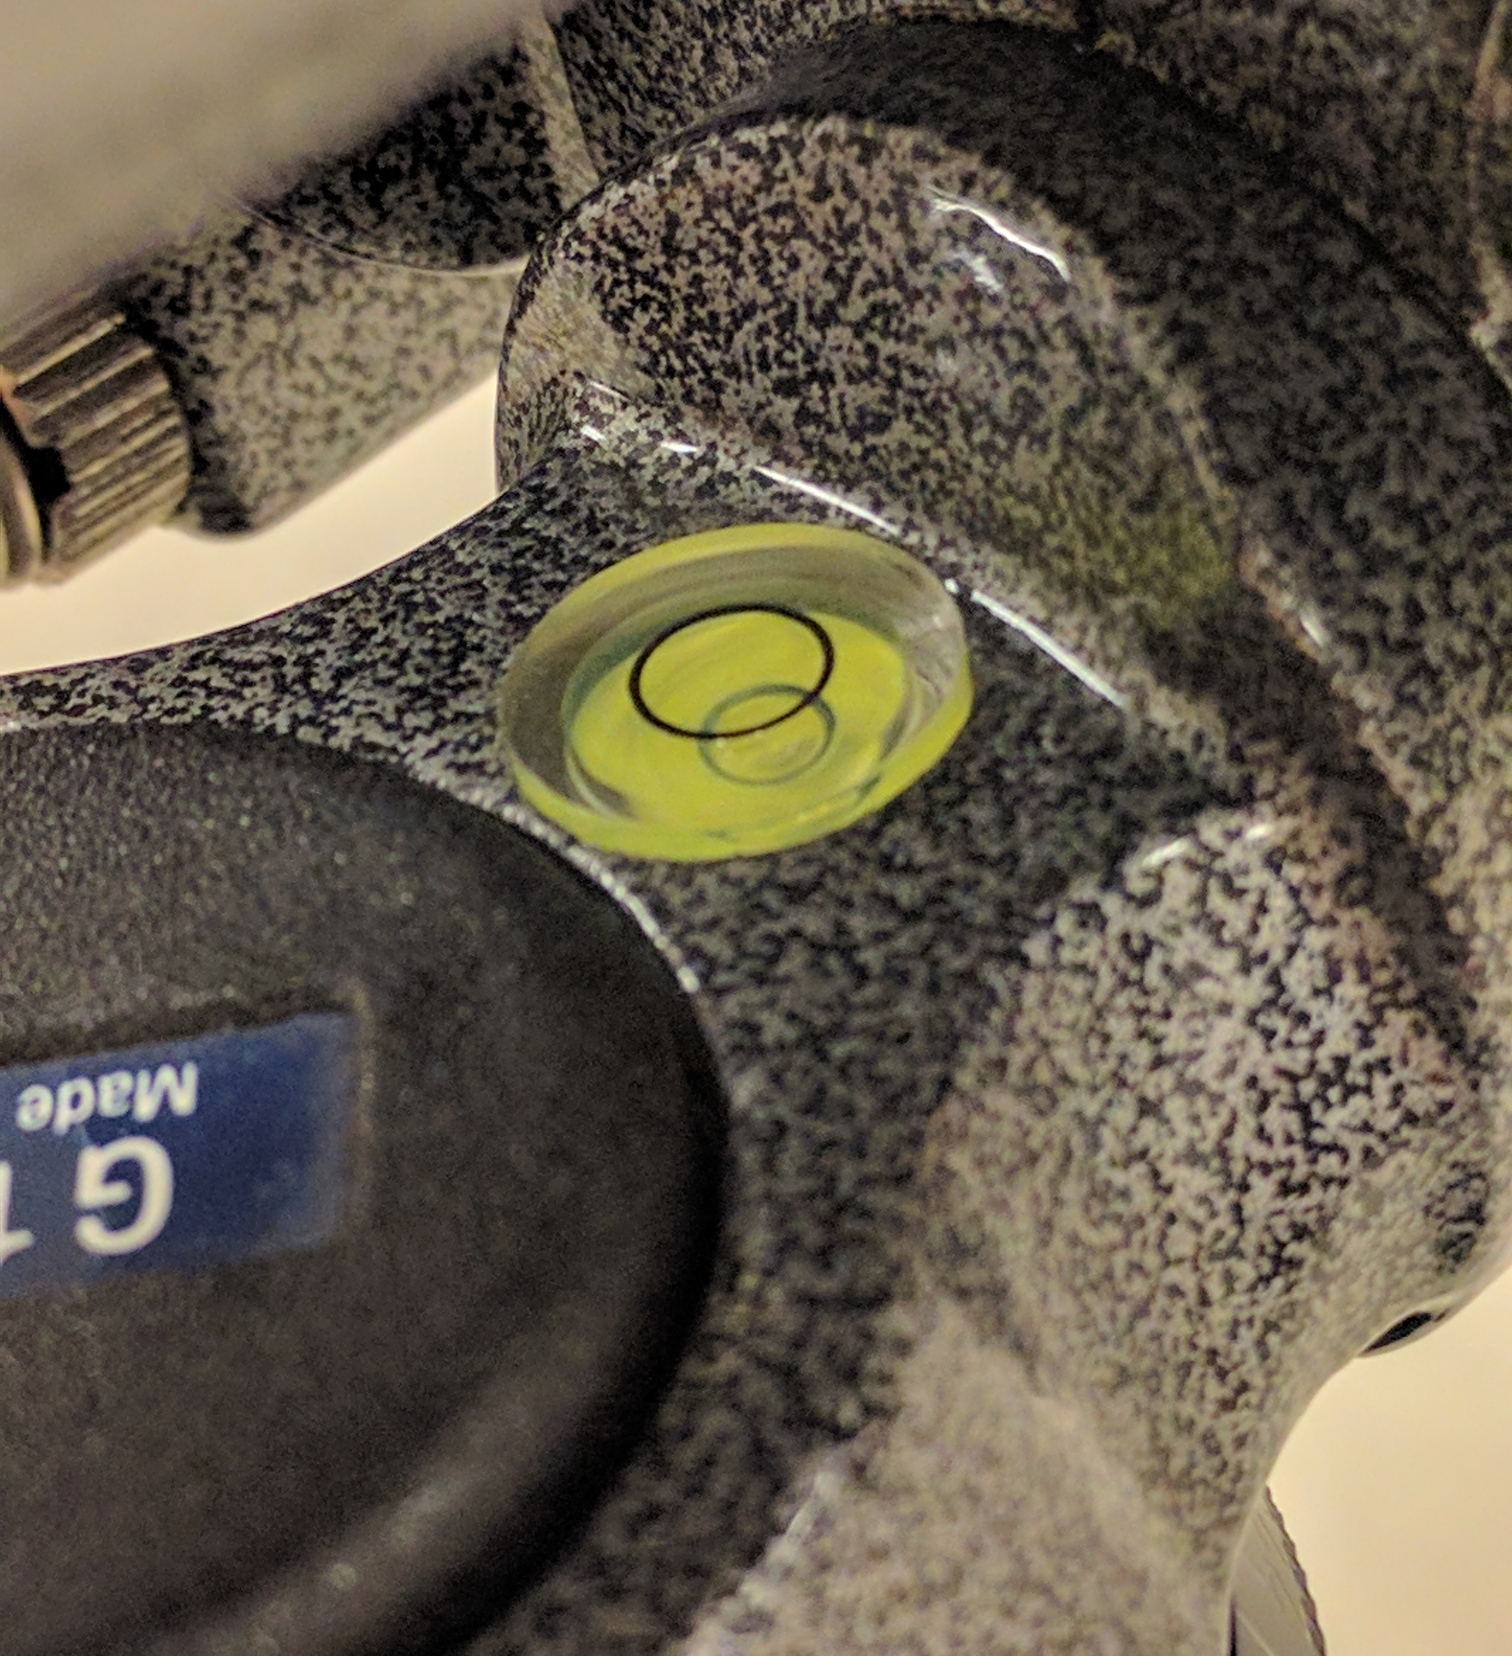
\includegraphics[width=0.5\textwidth]{fig/vater}
  \caption{Bulls eye spirit level on the tripod}
  \label{fig:vater}
\end{figure}


\subsubsection{Accuracy of mapping with accurate height measurement}
I want to test how accurate the system can map and calculate the wall lengths using a very accurate height measurement. Using the setup described previously, and omitting the measured height from the range sensor, and feeding an accurate height in the program, I can compare the calculated wall lengths with the actual wall lengths. \\

Since the range sensor has some inaccuracies, I measure the distance from the ground with a measuring tape. The measured height above the ground plane is:
\begin{align*}
Measured\_height = 162,3 \quad [cm]
\end{align*}
I have plotted the output of the algorithm when feeding the correct height over the image the algorithm captures:
\begin{figure}[H]
\centering
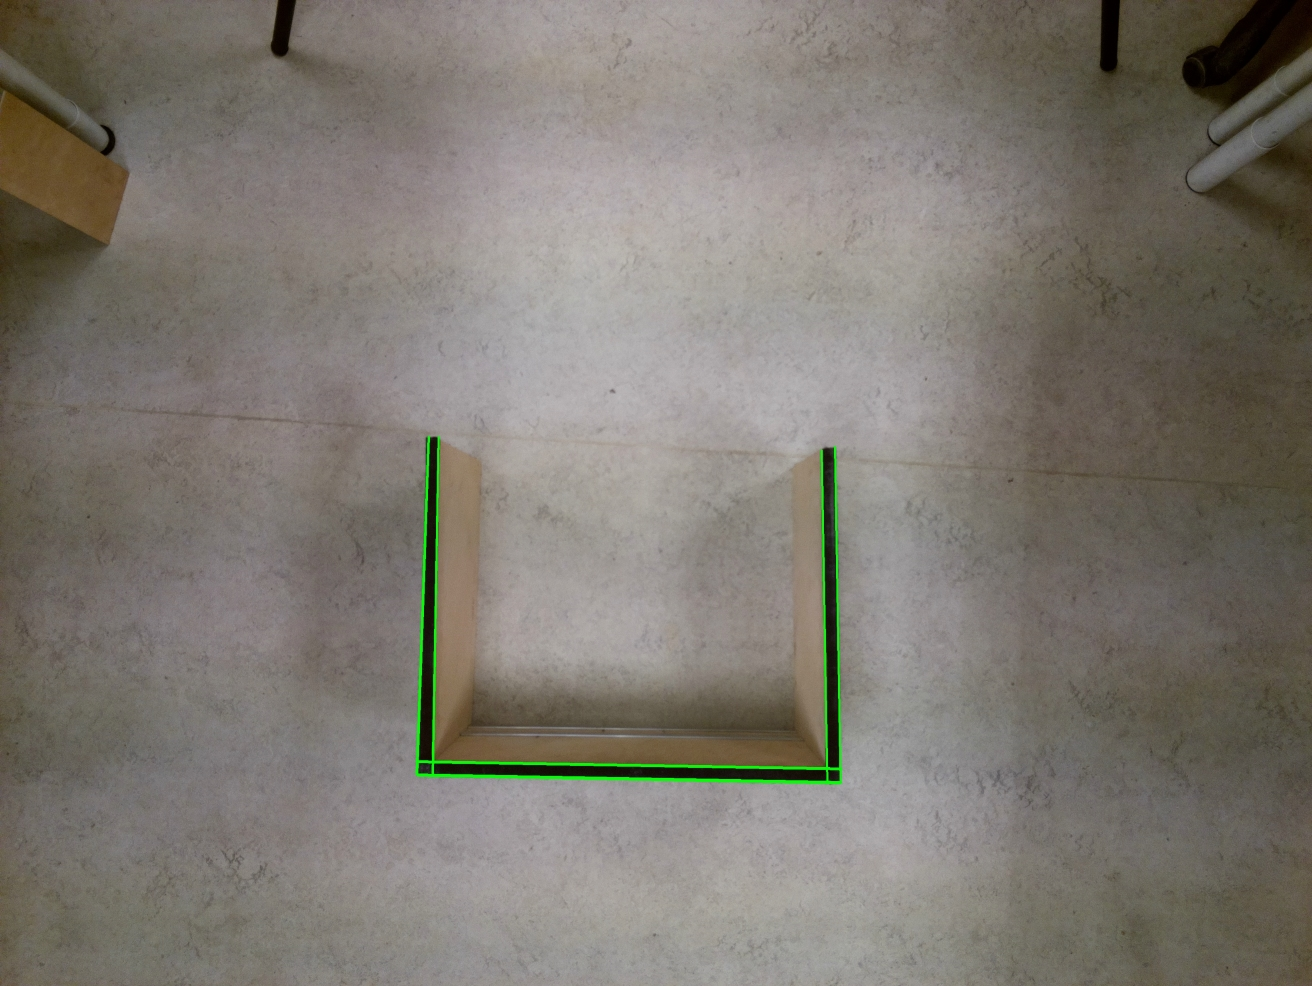
\includegraphics[width=0.8\textwidth]{fig/houghlines}
  \caption{Output from algorithm}
  \label{fig:houghlines}
\end{figure}

The algorithm also calculates the length of each detected wall segment and outputs them in the terminal, giving the following values in cm: 
\begin{align*}
[52.13614559709601, 
51.84253572745204, 
41.58182396984803,\\
41.454211626629274, 
40.893884097286644, 
52.13614559709601,\\
41.18835500372284, 
51.989768062876635,
52.08792302779498,\\
41.482826496385684,
41.40344063095725]
\end{align*}
A weakness in the algorithm, which I will explain later, is that the algorithm might detect the same wall several times, with slightly different length values. By sorting the values, by back wall and side walls, and taking the mean of each wall segment I get the following:
\begin{align*}
\textbf{Length Back Wall} = 52.04 \quad [cm]\\
\textbf{Length Side Wall} = 41.33 \quad [cm]
\end{align*}
I have the actual measurements of the test maze:
\begin{align*}
\textbf{Actual Length Back Wall} = 53.1 \quad [cm]\\
\textbf{Actual Length Side Wall} = 42.5 \quad [cm]
\end{align*}
Calculate the difference:
\begin{align*}
\Delta\textbf{Length Back Wall} = 53.1 - 52.04 = 1.06 \quad [cm]\\
\Delta\textbf{Length Side Wall} = 42.5 - 41.33 = 1.17 \quad [cm]
\end{align*}
In percent the differences are in terms of the actual value of the wall:
\begin{align*}
\Delta\textbf{Length Back Wall in \%} = \frac{1.06}{53.1} = 0.0199 = 2\% \\
\Delta\textbf{Length Side Wall in \%} = \frac{1.17}{42.5} = 0.0275 = 2.75\%
\end{align*}
The same test was done in Bjørnsen 2016\cite{kris}. In that implementation, the results was:
\begin{align*}
\Delta\textbf{Length Left Wall Bjørnsen 2016} = 42,2123-42,5 = -0,2887\quad [cm]\\
\Delta\textbf{Length Back Wall Bjørnsen 2016} = 53,5241-53,1 = 0,4241\quad [cm]\\
\Delta\textbf{Length Right Wall Bjørnsen 2016} = 43,0162-42,9 = 0,1162\quad [cm]
\end{align*}
All the calculated lengths in this older application was closer to the actual length than that in the current application written in Python. 





















